\documentclass[11pt,compress,t,notes=noshow, xcolor=table]{beamer}
\usepackage[]{graphicx}\usepackage[]{color}
% maxwidth is the original width if it is less than linewidth
% otherwise use linewidth (to make sure the graphics do not exceed the margin)
\makeatletter
\def\maxwidth{ %
  \ifdim\Gin@nat@width>\linewidth
    \linewidth
  \else
    \Gin@nat@width
  \fi 
}
\makeatother

\definecolor{fgcolor}{rgb}{0.345, 0.345, 0.345}
\newcommand{\hlnum}[1]{\textcolor[rgb]{0.686,0.059,0.569}{#1}}%
\newcommand{\hlstr}[1]{\textcolor[rgb]{0.192,0.494,0.8}{#1}}%
\newcommand{\hlcom}[1]{\textcolor[rgb]{0.678,0.584,0.686}{\textit{#1}}}%
\newcommand{\hlopt}[1]{\textcolor[rgb]{0,0,0}{#1}}%
\newcommand{\hlstd}[1]{\textcolor[rgb]{0.345,0.345,0.345}{#1}}%
\newcommand{\hlkwa}[1]{\textcolor[rgb]{0.161,0.373,0.58}{\textbf{#1}}}%
\newcommand{\hlkwb}[1]{\textcolor[rgb]{0.69,0.353,0.396}{#1}}%
\newcommand{\hlkwc}[1]{\textcolor[rgb]{0.333,0.667,0.333}{#1}}%
\newcommand{\hlkwd}[1]{\textcolor[rgb]{0.737,0.353,0.396}{\textbf{#1}}}%
\let\hlipl\hlkwb

\usepackage{framed}
\makeatletter
\newenvironment{kframe}{%
 \def\at@end@of@kframe{}%
 \ifinner\ifhmode%
  \def\at@end@of@kframe{\end{minipage}}%
  \begin{minipage}{\columnwidth}%
 \fi\fi%
 \def\FrameCommand##1{\hskip\@totalleftmargin \hskip-\fboxsep
 \colorbox{shadecolor}{##1}\hskip-\fboxsep
     % There is no \\@totalrightmargin, so:
     \hskip-\linewidth \hskip-\@totalleftmargin \hskip\columnwidth}%
 \MakeFramed {\advance\hsize-\width
   \@totalleftmargin\z@ \linewidth\hsize
   \@setminipage}}%
 {\par\unskip\endMakeFramed%
 \at@end@of@kframe}
\makeatother

\definecolor{shadecolor}{rgb}{.97, .97, .97}
\definecolor{messagecolor}{rgb}{0, 0, 0}
\definecolor{warningcolor}{rgb}{1, 0, 1}
\definecolor{errorcolor}{rgb}{1, 0, 0}
\newenvironment{knitrout}{}{} % an empty environment to be redefined in TeX

\usepackage{alltt}
\newcommand{\SweaveOpts}[1]{}  % do not interfere with LaTeX
\newcommand{\SweaveInput}[1]{} % because they are not real TeX commands
\newcommand{\Sexpr}[1]{}       % will only be parsed by R



\usepackage[english]{babel}
\usepackage[utf8]{inputenc}

\usepackage{dsfont}
\usepackage{verbatim}
\usepackage{amsmath}
\usepackage{amsfonts}
\usepackage{bm}
\usepackage{csquotes}
\usepackage{multirow}
\usepackage{longtable}
\usepackage{booktabs}
\usepackage{enumerate}
\usepackage[absolute,overlay]{textpos}
\usepackage{psfrag}
\usepackage{algorithm}
\usepackage{algpseudocode}
\usepackage{eqnarray}
\usepackage{arydshln}
\usepackage{tabularx}
\usepackage{placeins}
\usepackage{tikz}
\usepackage{setspace}
\usepackage{colortbl}
\usepackage{mathtools}
\usepackage{wrapfig}
\usepackage{bm}
\usepackage{xcolor}
\usetikzlibrary{shapes,arrows,automata,positioning,calc,chains,trees, shadows}
\tikzset{
  %Define standard arrow tip
  >=stealth',
  %Define style for boxes
  punkt/.style={
    rectangle,
    rounded corners,
    draw=black, very thick,
    text width=6.5em,
    minimum height=2em,
    text centered},
  % Define arrow style
  pil/.style={
    ->,
    thick,
    shorten <=2pt,
    shorten >=2pt,}
}
\usepackage{subfig}


% Defines macros and environments
\input{../../style/common.tex}

%\usetheme{lmu-lecture}
% \newcommand{\titlefigure}{figure/ml-basic-riskmin-error-surface.png}
% \newcommand{\learninggoals}{\item Know the concept of loss \item Understand the relationship between loss and risk \item Understand the relationship between risk minimization and finding the best model}
\usepackage{fancy}

\colorlet{GRAY}{gray}

\let\code=\texttt
\let\proglang=\textsf

\setkeys{Gin}{width=0.9\textwidth}

\title{Introduction to Machine Learning}
% \author{Bernd Bischl, Christoph Molnar, Daniel Schalk, Fabian Scheipl}
\institute{\href{https://compstat-lmu.github.io/lecture_i2ml/}{compstat-lmu.github.io/lecture\_i2ml}}
\date{}

\setbeamertemplate{frametitle}{\expandafter\uppercase\expandafter\insertframetitle}



\begin{document}
% Introduction to Machine Learning
% Day 1

% Set style/preamble.Rnw as parent.

% Load all R packages and set up knitr

% This file loads R packages, configures knitr options and sets preamble.Rnw as parent file
% IF YOU MODIFY THIS, PLZ ALSO MODIFY setup.Rmd ACCORDINGLY...








% Defines macros and environments
\input{../../latex-math/basic-math.tex}
\input{../../latex-math/basic-ml.tex}
\input{../../latex-math/ml-lm.tex}

%! includes: basics-learners

\lecturechapter{ML-Basics: Losses \& Risk Minimization}
\lecture{Introduction to Machine Learning}

\begin{vbframe}{How to Evaluate Models}


 \end{vbframe}

\begin{frame}{Overview}

No Free Lunch
In machine learning, there’s something called the “No Free Lunch” theorem. In a nutshell, it states that no one algorithm works best for every problem, and it’s especially relevant for supervised learning (i.e. predictive modeling).

For example, you can’t say that neural networks are always better than decision trees or vice-versa. There are many factors at play, such as the size and structure of your dataset.

As a result, you should try many different algorithms for your problem, while using a hold-out “test set” of data to evaluate performance and select the winner.
\lz
\lz
Hypothesisspace + Risk + Optimization 
\end{frame}

% ------------------------------------------------------------------------------
% CART (Classification and Regression Trees)
% ------------------------------------------------------------------------------

\LARGE
\begin{frame}{\textcolor{gray!80}{CART} ~~ Functionality}
\normalsize
\vspace{-0.5cm}
\noindent \textcolor{gray!80}{\rule{\textwidth}{1pt}}

\vspace{0.2cm}

\scriptsize

\colorbox{gray!80}{\textcolor{white}{NON-PARAMETRIC}} 
\colorbox{gray!80}{\textcolor{white}{WHITE-BOX}} 
\colorbox{gray!80}{\textcolor{white}{FEATURE SELECTION}}

\medskip

\textbf{\textcolor{gray!80}{General idea}} {}{} Starting from a root node, 
\textit{\textbf{classification \& regression trees (CART)}} 
perform repeated \textbf{binary splits} of the data according to feature values, 
thereby subsequently dividing the input space $\Xspace$ into $M$ 
\textbf{rectangular partitions}.

\begin{itemize}
  \item [$\rightarrow$] Pass observations along until each ends up in exactly 
  one leaf node
  \item [$\rightarrow$] In each step, find the optimal feature-threshold
  combination to split by
  \item [$\rightarrow$] Assign response $c_m$ to leaf node $m$
\end{itemize}

\vspace{0.1cm}

\begin{minipage}{0.6\textwidth}
  \textbf{\textcolor{gray!80}{Hypothesis space}} \\
  $$\Hspace = \left\{ \fx: \fx = \sum_{m = 1}^M c_m \mathbb{I}(\xv \in Q_m) 
  \right\}$$
  \medskip
  \textbf{\textcolor{gray!80}{Loss functions}} \\
  Classification: mostly \textit{\textbf{Brier score, Bernoulli loss}}  \\
  \medskip
  Regression: mostly \textit{\textbf{quadratic loss}}
\end{minipage}%
\begin{minipage}{0.4\textwidth}
  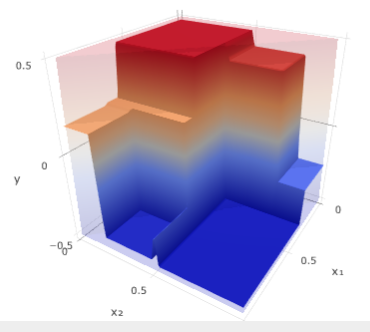
\includegraphics[width=0.8\textwidth]{figure/cart_3d.PNG}
\end{minipage}

\medskip
\textbf{\textcolor{gray!80}{Optimization}} {}{} Exhaustive search for optimal 
splitting criterion (greedy optimization) \\
\medskip
\textbf{\textcolor{gray!80}{Hyperparameters}} {}{} Tree depth, minimum number
of observations per node, ...

\vfill



\end{frame}

% % ------------------------------------------------------------------------------

\LARGE
\begin{frame}{\textcolor{gray!80}{CART} ~~ Pro's \& Con's}
\normalsize
\vspace{-0.5cm}
\noindent \textcolor{gray!80}{\rule{\textwidth}{1pt}}

\vspace{0.3cm}

\begin{columns}[onlytextwidth]
  \begin{column}{0.5\textwidth}
    \textbf{\textcolor{gray!80}{Advantages}}
    \footnotesize
    \begin{itemize}
      \item[$\textbf{\textcolor{gray!80}{+}}$] \textbf{Easy} to understand, 
      interpret \& visualize
      \item[$\textbf{\textcolor{gray!80}{+}}$] Automatic handling of 
      \textbf{non-numerical} features
      \item[$\textbf{\textcolor{gray!80}{+}}$] Built-in \textbf{feature 
      selection}
      \item[$\textbf{\textcolor{gray!80}{+}}$] Automatic handling of 
      \textbf{missings} 
      \item[$\textbf{\textcolor{gray!80}{+}}$] \textbf{Interaction} effects 
      between features easily possible, even of higher orders
      \item[$\textbf{\textcolor{gray!80}{+}}$] \textbf{Fast} computation and 
      good scalability
      \item[$\textbf{\textcolor{gray!80}{+}}$] High \textbf{flexibility} (custom 
      split criteria or leaf-node prediction rules)   
    \end{itemize}
  \end{column}
  \begin{column}{0.5\textwidth}
    \textbf{\textcolor{gray!80}{Disadvantages}}
    \footnotesize
    \begin{itemize}
      \item[$\textbf{\textcolor{gray!80}{-}}$] Rather \textbf{low accuracy} (at least, 
      without bagging or boosting)
      \item[$\textbf{\textcolor{gray!80}{-}}$] High \textbf{variance/instability}: strong 
      dependence on training data
      \item[$\textbf{\textcolor{gray!80}{-}}$] Therefore, poor generalization \& 
      risk of \textbf{overfitting}
      \item[$\textbf{\textcolor{gray!80}{-}}$] Several steps required for
      modeling linear relationships
      \item[$\textbf{\textcolor{gray!80}{-}}$] In presence of categorical 
      features, \textbf{bias} towards features with \textbf{many categories}
    \end{itemize}
  \end{column}
\end{columns}

\vfill

\small

\fbox{\parbox{\textwidth}{
\centering
\textbf{Simple and good with feature selection, but not the best
predictor}}}

\end{frame}

% ------------------------------------------------------------------------------

\LARGE
\begin{frame}{\textcolor{gray!80}{CART} ~~ Application}
\normalsize
\vspace{-0.5cm}
\noindent \textcolor{gray!80}{\rule{\textwidth}{1pt}}

\vspace{0.3cm}

\textbf{For applications of CART, note the following:}
\lz

\textbf{\textcolor{gray!80}{Pruning / early stopping}} \\
\smallskip
Unless interrupted, splitting will go on until each leaf node contains a single 
observation (expensive + overfitting!) \\
\smallskip
$\rightarrow$ Use \textbf{pruning} and \textbf{stopping criteria} to limit 
complexity.

\lz
\textbf{\textcolor{gray!80}{Implementation}} \\
\smallskip
R: package \texttt{rpart}\\
Python: \texttt{DecisionTreeClassifier} from package \texttt{scikit-learn}

\lz
\textbf{\textcolor{gray!80}{Bagging}} \\
\smallskip
Since CART are instable predictors on their own, they are typically ensembled
to form a \textbf{random forest}.

\end{frame}

% ------------------------------------------------------------------------------

\endlecture

\end{document}
